% This LaTeX document needs to be compiled with XeLaTeX.
\documentclass[10pt]{article}
\usepackage[utf8]{inputenc}
\usepackage{ucharclasses}
\usepackage{amsmath}
\usepackage{amsfonts}
\usepackage{amssymb}
\usepackage[version=4]{mhchem}
\usepackage{stmaryrd}
\usepackage{graphicx}
\usepackage[export]{adjustbox}
\graphicspath{ {./images/} }
\usepackage{bbold}
\usepackage{hyperref}
\hypersetup{colorlinks=true, linkcolor=blue, filecolor=magenta, urlcolor=cyan,}
\urlstyle{same}
\usepackage{polyglossia}
\usepackage{fontspec}
\usepackage{newunicodechar}
\setmainlanguage{english}
\setotherlanguages{french, thai}
\IfFontExistsTF{Noto Serif Thai}
{\newfontfamily\thaifont{Noto Serif Thai}}
{\IfFontExistsTF{Thonburi}
  {\newfontfamily\thaifont{Thonburi}}
  {\IfFontExistsTF{FreeSerif}
    {\newfontfamily\thaifont{FreeSerif}}
    {\IfFontExistsTF{Tahoma}
      {\newfontfamily\thaifont{Tahoma}}
      {\newfontfamily\thaifont{Arial Unicode MS}}
}}}
\IfFontExistsTF{CMU Serif}
{\newfontfamily\lgcfont{CMU Serif}}
{\IfFontExistsTF{DejaVu Sans}
  {\newfontfamily\lgcfont{DejaVu Sans}}
  {\newfontfamily\lgcfont{Georgia}}
}
\setDefaultTransitions{\lgcfont}{}
\setTransitionsFor{Thai}{\thaifont}{\lgcfont}

%New command to display footnote whose markers will always be hidden
\let\svthefootnote\thefootnote
\newcommand\blfootnotetext[1]{%
  \let\thefootnote\relax\footnote{#1}%
  \addtocounter{footnote}{-1}%
  \let\thefootnote\svthefootnote%
}

%Overriding the \footnotetext command to hide the marker if its value is `0`
\let\svfootnotetext\footnotetext
\renewcommand\footnotetext[2][?]{%
  \if\relax#1\relax%
    \ifnum\value{footnote}=0\blfootnotetext{#2}\else\svfootnotetext{#2}\fi%
  \else%
    \if?#1\ifnum\value{footnote}=0\blfootnotetext{#2}\else\svfootnotetext{#2}\fi%
    \else\svfootnotetext[#1]{#2}\fi%
  \fi
}

\newunicodechar{⟹}{\ifmmode\Longrightarrow\else{$\Longrightarrow$}\fi}

\begin{document}
\section*{Literature and Strategy Report for the Alaoglu-Erdős Integer-Exponent Conjecture}
\section*{Executive summary}
I audited the attached TeX report, including its bibliography and full text, before searching the literature. The report is already unusually strong on the four-/five-/six-exponentials side: it knows the four-exponentials reduction, Gelfond-Schneider, Baker's homogeneous theorem, Roy's strong/sharp six-exponentials results, the exact conditional monoid generated by a least counterexample, radical/Kummer reformulations, rational-third-base reductions, arbitrary-node and generalized-Vandermonde determinant methods, finite differences, a compact $S$-integral orbit, and the sufficient "prime-log-product independence" condition implied by Schanuel. It also explicitly diagnoses the central obstacle

$$
\log M \log 3-\log A \log 2=0, \quad M=2^{\beta}, \quad A=3^{\beta},
$$

as a bilinear relation between logarithms, outside the usual scope of Baker-type linear forms.

The largest gaps I found are elsewhere. The report contains no substantive use or citation of the quantitative $S$-unit/Subspace-Theorem literature of Evertse-Schlickewei-Schmidt and Corvaja-Zannier; no Matveev, Baker-Wüstholz, Gouillon, or modern explicit $p$-adic logarithmic-form results; no Mahler-Pisot/ Subspace-Theorem classification of powers exponentially close to integers; no Hadamard-quotient/integral-value theory for recurrence sequences; and no modern integer-valued o-minimal results. Pila-Wilkie is discussed generically, but its important primary literature and the 2024-2026 breakthroughs on polylogarithmic/effective counting are uncited. "Laurent's interpolation-determinant method" is mentioned once in an experimental suggestion, but the Laurent-Mignotte-Nesterenko and Laurent papers developing that method are not cited or exploited.

My main conclusion is that three additions to the current program deserve substantially higher priority than the rest.

First, the conditional counterexample has an arithmetic-geometric formulation stronger than the report presently exploits. If

$$
M=2^{\beta}, \quad A=3^{\beta}
$$

are integers for an irrational $\beta$, define

$$
r_{k}=\lfloor k \beta\rfloor, \quad P_{k}=\left(\frac{M^{k}}{2^{r_{k}}}, \frac{A^{k}}{3^{r_{k}}}\right)=\left(2^{\{k \beta\}}, 3^{\{k \beta\}}\right) .
$$

Then every $P_{k}$ lies simultaneously

$$
P_{k} \in \Gamma=\left\langle(M, A),\left(2^{-1}, 3^{-1}\right)\right\rangle \subset \mathbf{G}_{m}^{2}(\mathbf{Q}),
$$

where $\Gamma$ has rank at most two, and

$$
P_{k} \in \mathcal{C}=\left\{\left(u, u^{\theta}\right): 1 \leq u<2\right\}, \quad \theta=\frac{\log 3}{\log 2} .
$$

Moreover, logarithmic height grows linearly with $k$. Thus a counterexample produces $\asymp T$ points of logarithmic height at most $T$ in the intersection of a fixed rank-two multiplicative group with a fixed transcendental Pfaffian arc. The Evertse-Schlickewei-Schmidt theorem gives extremely strong control once points are forced onto algebraic curves, while the newest Pila-Wilkie/Pfaffian methods control how transcendental sets can be covered or populated by algebraic/rational points. 1 This suggests a very concrete missing theorem:

$$
\#\{P \in \Gamma \cap \mathcal{C}: h(P) \leq T\}=o(T)
$$

for this particular rank-two $\Gamma$ and arc-or even a sufficiently strong special case exploiting the synchronized denominator vector $\left(2^{r_{k}}, 3^{r_{k}}\right)$. Proving this would settle the conjecture. Existing general o-minimal counting is not yet strong enough, but the combination of algebraic covering + finite-rank multiplicative rigidity + synchronized denominators appears not to have been exhausted.

Second, the determinant program should be rebuilt using the technology of interpolation determinants rather than only ordinary/generalized Vandermonde determinants. Laurent-Mignotte-Nesterenko introduced a determinant construction specifically to squeeze arithmetic lower bounds and analytic upper bounds simultaneously, and Laurent refined it further in 2008. 2 This is unusually close to the attached report's quantitative bottleneck. The report currently needs approximately $(\log X)^{2}$ nodes where the hypothetical counterexample supplies only $\asymp \log X$. Interpolation determinants, multiplicities/confluent columns, zero lemmas, asymmetric monomial sets, and arithmetic row/column transformations are precisely the machinery designed to improve such parameter balances. This does not mean that an existing Laurent theorem proves the conjecture; rather, the report's determinant architecture currently uses only a restricted subset of the known design space.

Third, the report's proposed $p$-adic amplification should be made much more concrete. Recent explicit work of Chim gives sharp bounds for two $p$-adic logarithms with only $\log B$ dependence in the exponent parameter, improving the older $(\log B)^{2}$ behavior in the relevant two-log setting; Palojärvi-Seppälä and Gaudron provide complementary explicit and simultaneous archimedean/ $p$-adic frameworks. ${ }^{3}$ These theorems do not directly supply the large divisibility the report wants-they principally prevent excessive $p$ -adic cancellation-but that is exactly useful after a tropical/min-plus valuation argument has supplied a forced common factor: they can bound the extra cancellation among determinant terms and may permit a clean product-formula argument.

A second tier of literature is highly relevant if one can manufacture an appropriate auxiliary sequence. Corvaja-Zannier's results on integral values of quotients of linear recurrences, power sums, and exponentially good approximation of algebraic powers are powerful "structure from infinitely many arithmetic coincidences" theorems. 4 At present the missing step is to derive from $2^{\beta}, 3^{\beta} \in \mathbf{Z}$ an infinite family of the exact arithmetic events to which these theorems apply. Finding such an auxiliary quotient or\\
power sum should be an explicit computational research objective rather than dismissed as merely adjacent theory.

Finally, modern model theory gives an instructive negative result. Bays-Kirby-Wilkie prove a Schanuel-type property for exponentially transcendental power parameters. 5 But

$$
\theta=\frac{\log 3}{\log 2}
$$

is itself exponentially algebraic: $(z, w)=(\log 2, \theta)$ is a nonsingular solution of

$$
e^{z}-2=0, \quad e^{z w}-3=0,
$$

whose Jacobian determinant is $6 \log 2$ / 0 . Thus the most powerful "generic power" model-theoretic results deliberately exclude exactly the exceptional parameter occurring here. This explains why generic o-minimal/ model-theoretic methods should be treated as structural guides rather than expected black-box proofs.

The prioritized picture is therefore:

\begin{center}
\begin{tabular}[t]{|l|l|l|}
\hline
Priority & Direction & Assessment \\
\hline
Highest & Rank-two multiplicative group + specialized o-minimal/algebraic covering + S-unit rigidity & Most promising genuinely new synthesis \\
\hline
Highest & Laurent-style interpolation determinant redesign of the report's semigroup determinant & Closest existing technology to the identified missing $\log X$ factor \\
\hline
Highest & Tropical/ $p$-adic determinant amplification, with modern $p$-adic logarithmic-form control & Directly targets Priority A in the report \\
\hline
High & Corvaja-Zannier recurrence/powersum machinery after manufacturing an integral quotient & Potentially decisive if the right auxiliary sequence is found \\
\hline
High & Mahler-Ridout-Corvaja-Zannier exponential-nearness criterion & Gives a sharp conditional target: construct one non-Pisot algebraic power sequence exponentially close to integers \\
\hline
Medium & Matveev/Laurent/Gouillon/ Mignotte-Voutier effective logarithmic forms & Excellent for finite verification and auxiliary lemmas; unlikely to cross the fundamental bilinear barrier alone \\
\hline
Medium & Integer-valued o-minimal functions & Methodologically very close to the determinant/ integrality problem; existing theorem does not directly fit the sparse multiplicative grid \\
\hline
\end{tabular}
\end{center}

\begin{center}
\begin{tabular}[t]{|l|l|l|}
\hline
Priority & Direction & Assessment \\
\hline
Low as a direct attack & Skolem-Mahler-Lech, generic power model theory, general Zilber-Pink & Useful after an algebraization/recurrence bridge; currently one abstraction layer too far away \\
\hline
\end{tabular}
\end{center}

\section*{What the literature adds to the present reduction}
The basic obstruction can be phrased in several equivalent currencies, and the newly located literature attaches to different currencies.

A nontrivial counterexample must give integers $M, A>1$ with

$$
\beta=\frac{\log M}{\log 2}=\frac{\log A}{\log 3} \notin \mathbf{Z},
$$

hence


\begin{equation*}
\log M \log 3=\log A \log 2 . \tag{1}
\end{equation*}


For rational $\beta=a / b$ in lowest terms, $2^{a / b} \in \mathbf{Z}$ forces $b=1$ by prime valuations, so a counterexample is necessarily irrational. The standard four-exponentials formulation is therefore genuinely the correct transcendence-theoretic level rather than an artifact of presentation.

The attached report goes significantly farther conditionally: choosing a least positive nonintegral solution $\beta$ gives the two-generator solution lattice/monoid. That structure should be regarded as a major asset, because most transcendence literature treats arbitrary algebraic numbers whereas here every hypothetical solution comes with the same two integer generators $M, A$.

The most useful normalization for the newly found literature is


\begin{equation*}
P_{k}=\left(U_{k}, V_{k}\right)=\left(M^{k} 2^{-\lfloor k \beta\rfloor}, A^{k} 3^{-\lfloor k \beta\rfloor}\right) . \tag{2}
\end{equation*}


There are three simultaneous structures here.

First, analytically,

$$
\left(U_{k}, V_{k}\right)=\left(2^{t_{k}}, 3^{t_{k}}\right), \quad t_{k}=\{k \beta\},
$$

so the points lie on the real-analytic arc


\begin{equation*}
\mathcal{C}: \quad v=u^{\theta}, \quad \theta=\log _{2} 3 . \tag{3}
\end{equation*}


Second, arithmetically,


\begin{equation*}
\left(U_{k}, V_{k}\right) \in \Gamma=\left\langle(M, A),\left(2^{-1}, 3^{-1}\right)\right\rangle, \tag{4}
\end{equation*}


a finitely generated subgroup of $\mathbf{G}_{m}^{2}(\mathbf{Q})$ of rank at most two.

Third, the denominators are not arbitrary points of $\Gamma$. They have the synchronized form


\begin{equation*}
\operatorname{den}\left(U_{k}\right)=2^{r_{k}} / \operatorname{gcd}\left(M^{k}, 2^{r_{k}}\right), \quad \operatorname{den}\left(V_{k}\right)=3^{r_{k}} / \operatorname{gcd}\left(A^{k}, 3^{r_{k}}\right), \quad r_{k}=\lfloor k \beta\rfloor . \tag{5}
\end{equation*}


That common integer $r_{k}$ is information thrown away by ordinary Pila-Wilkie height counting.

This gives the following logical map.\\
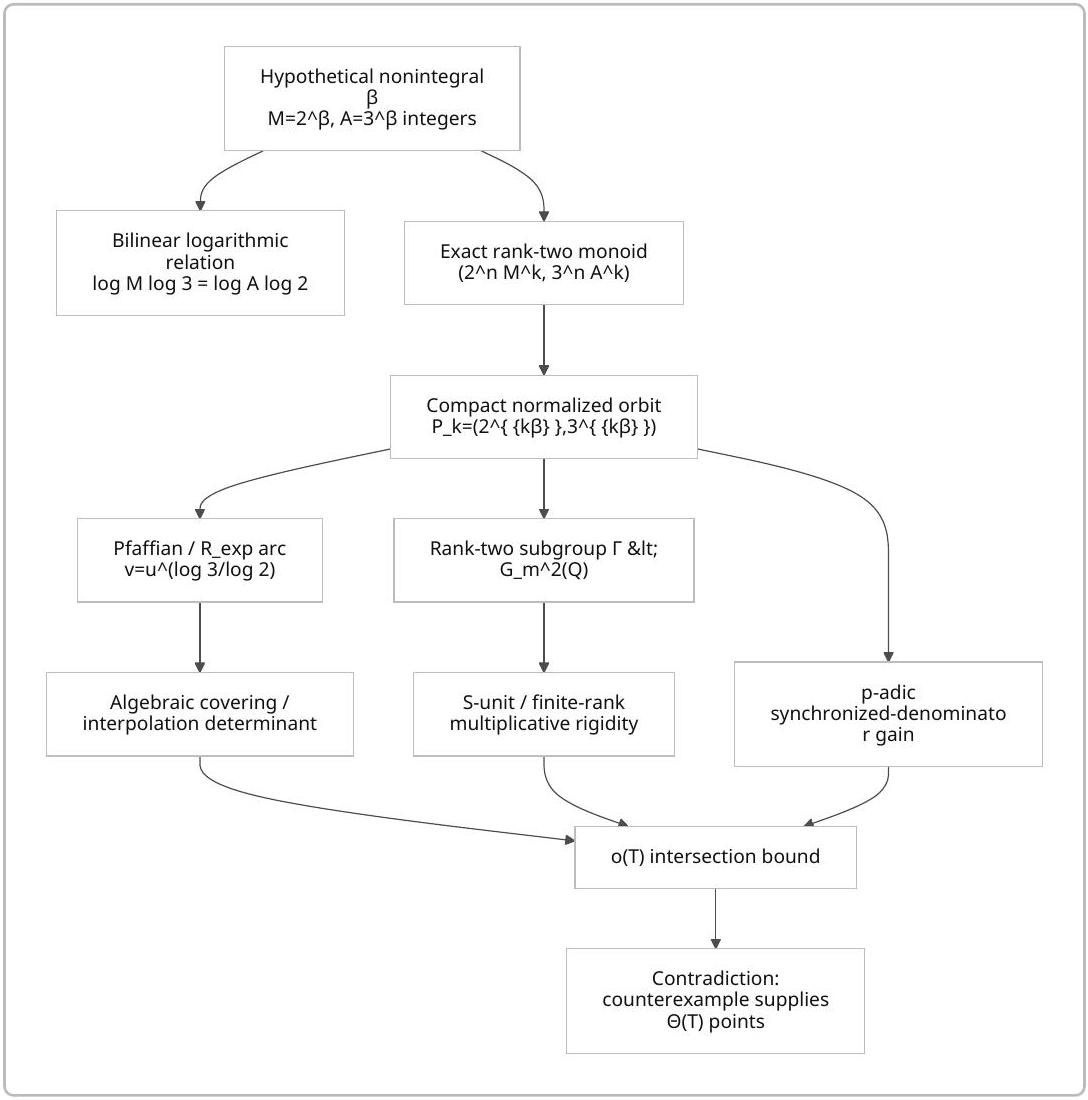
\includegraphics[max width=\textwidth, alt={}, center]{14655053-5393-4a14-bc7a-9901afeb0814-05_1100_1088_724_518}\\
This formulation clarifies why several famous theorems are tantalizing but insufficient by themselves.

The Evertse-Schlickewei-Schmidt theorem says that, in a finite-rank multiplicative group, a fixed linear equation has only boundedly many nondegenerate solutions, with a bound depending only on the number of variables and the group's rank. 6 Applied to a sparse Laurent polynomial

$$
F(X, Y)=\sum_{j=1}^{s} c_{j} X^{a_{j}} Y^{b_{j}}
$$

the monomials evaluated on $\Gamma$ again lie in a finite-rank multiplicative group, so $F(P)=0$ becomes an $S$ -unit-type equation. Thus any procedure that forces many $P_{k}$ 's onto one fixed sparse algebraic curve immediately gains a powerful second-stage theorem. Degenerate subsums correspond to lower-support equations and, ultimately, binomial/toric exceptional sets.

Those exceptional binomials are especially harmless on this particular arc. A torus coset has an equation

$$
u^{a} v^{b}=c .
$$

On $u=2^{t}, v=3^{t}$, this becomes

$$
e^{t(a \log 2+b \log 3)}=c .
$$

For $(a, b) /(0,0)$, multiplicative independence of 2,3 makes $a \log 2+b \log 3 / 0$, so such a coset meets the real arc in at most one point. In other words, the usual "special subvarieties" that complicate Mordell-Lang-type statements do not look capable of hosting the hypothetical orbit. This is one reason the rank-two-group formulation seems materially stronger than generic rational-point counting.

The modern point-counting side has also moved significantly beyond what is reflected in the report. Binyamini-Novikov-Zak proved an effective polylogarithmic form of Wilkie's conjecture for Pfaffian structures and deduced Wilkie's conjecture for the full real exponential field: rational points of multiplicative height $H$ on the transcendental part have cardinality bounded by a power of $\log H$. 7 Binyamini-Jones-Schmidt-Thomas have since obtained an effective Pila-Wilkie theorem for Pfaffian-definable sets with effective algebraic-point bounds and strong uniformity in complexity; that paper appeared online in April 2026. 8 Pila's earlier paper proves Wilkie-type counting for a particular exponential-algebraic surface, and its published correction explicitly states that all theorems remain valid. ${ }^{9}$

Unfortunately, translating multiplicative height $H$ to logarithmic height $T=\log H$ turns a bound $(\log H)^{C}$ into $T^{C}$. A hypothetical Alaoglu-Erdős orbit contributes $\asymp T$ points. Thus a generic exponent $C>1$ does not contradict it. The exact target is not "apply Pila-Wilkie," but instead obtain an exponent below one, or exploit the rank-two/denominator structure to remove an extra factor.

That observation turns the report's "denominator-sensitive counting" priority into a much sharper research problem:

Rank-two Pfaffian intersection problem. For the fixed $\operatorname{arc} \mathcal{C}=\left\{\left(2^{t}, 3^{t}\right): 0 \leq t<1\right\}$, a rank-two subgroup

$$
>\Gamma=\left\langle(M, A),\left(2^{-1}, 3^{-1}\right)\right\rangle \subset \mathbf{G}_{m}^{2}(\mathbf{Q}),>
$$

and points satisfying the synchronized denominator condition (5), prove

$$
>N_{\Gamma}(T)=o(T) .>
$$

A weaker but still sufficient version could count only the one-parameter subsequence in (2), rather than all of $\Gamma$.

There is an important possible route from the point-counting theorem to the $S$-unit theorem: algebraic covering followed by finite-rank rigidity. Binyamini-Novikov's complex-analytic proof of Pila-Wilkie explicitly reconnects rational-point counting with Bombieri-Pila interpolation determinants and algebraic hypersurface coverings. ${ }^{10}$ The missing optimization would be to force a set of $\asymp T$ synchronized points onto $o(T)$ algebraic curves of a controlled sparse type. Once the number of monomials is fixed, Evertse-

Schlickewei-Schmidt supplies a height-independent second-stage bound for nondegenerate points. ${ }^{6}$ This "cover first, $S$-unit second" strategy seems substantially more tailored to the conditional structure than invoking either theorem separately.

\section*{Prioritized references absent from the report}
The table below distinguishes absent works from sources whose general theme is named in the report but whose actual primary reference and machinery are not used.

\begin{center}
\begin{tabular}[t]{|l|l|l|l|l|}
\hline
Priority & Reference & Method & Why it matters here & Audit status \\
\hline
A+ & Evertse-SchlickeweiSchmidt, 20026 & Finite-rank multiplicative groups; $S$-unit equations & Controls algebraic relations among points of the conditional rank-two group; natural second stage after an interpolation covering & Entirely absent \\
\hline
A+ & Laurent-MignotteNesterenko, 1995 11 & Interpolation determinants; zero lemma; two logarithms & The closest established determinant architecture to the report's quantitative $\log X$ deficit & Laurent's method named once; paper absent \\
\hline
A+ & Laurent, 200812 & Refined interpolation determinants & Modern refinement of the preceding determinant design & Paper absent \\
\hline
A+ & Binyamini-Novikov-Zak, 2024 7 & Polylogarithmic rational-point counting in Pfaffian/ $\mathbb{R}_{\text {exp }}$ structures & Direct upgrade to the report's generic Pila-Wilkie discussion & Pila-Wilkie named; work absent \\
\hline
A+ & Binyamini-Jones-Schmidt-Thomas, 20268 & Effective Pila-Wilkie, effective Pfaffian parameterization & Current state of the art; possible vehicle for denominator/ranksensitive refinements & Entirely absent \\
\hline
A+ & Chim, 202513 & Explicit two- $p$-adiclog lower bounds & Most directly relevant recent input to the report's $p$-adic determinant program & Entirely absent \\
\hline
A & Corvaja-Zannier, 2002, Some New Applications... 14 & Subspace Theorem; $S$-unit points; power sums & Template for deriving rigidity from infinitely many integral/smallheight values & Entirely absent \\
\hline
\end{tabular}
\end{center}

\begin{center}
\begin{tabular}[t]{|l|l|l|l|l|}
\hline
Priority & Reference & Method & Why it matters here & Audit status \\
\hline
A & Corvaja-Zannier, 2002, recurrence quotients ${ }^{15}$ & Integral values of ratios of recurrences & Potentially decisive if a determinant/divideddifference quotient is found & Entirely absent \\
\hline
A & Corvaja-Zannier, 200416 & Mahler/Pisot problem via Subspace Theorem & Classifies algebraic powers exponentially close to integers; gives a sharp bridge lemma to seek & Entirely absent \\
\hline
A & Bhardwaj-McCulloch-RamachandranWoo, 202517 & Integer-valued $\mathbb{R}_{\text {an,exp }}$-definable functions & Methodologically almost tailor-made for "definability + determinant + integrality"; suggests sparse-grid analogues & Entirely absent \\
\hline
A- & Evertse-Ferretti, 201318 & Quantitative Subspace Theorem, height intervals & Useful if an auxiliary Subspace-Theorem inequality can be produced; provides quantitative height distribution & Entirely absent \\
\hline
A- & Palojärvi-Seppälä, 202319 & Explicit $p$-adic logarithmic forms & Complementary explicit technology for $p$-adic determinant cancellation & Entirely absent \\
\hline
A- & Gaudron, 201020 & Simultaneous archimedean/ $p$-adic logarithmic forms; adelic slopes & Conceptually relevant to a genuine product-formula determinant & Entirely absent \\
\hline
B+ & Baker-Wüstholz, 199321 & Explicit/general logarithmic forms on group varieties & Modernizes the report's Baker-1975 baseline; useful for effective auxiliary lemmas & Entirely absent \\
\hline
B+ & Matveev, 200022 & Explicit $n$-logarithm lower bounds & Standard computational engine for exponential Diophantine problems; valuable for finite ranges and auxiliary equations & Entirely absent \\
\hline
B+ & Gouillon, 200623 & Sharper explicit twolog bounds & Better suited than generic Matveev when only $M, 2$ or $A, 3$ occur & Entirely absent \\
\hline
\end{tabular}
\end{center}

\begin{center}
\begin{tabular}[t]{|l|l|l|l|l|}
\hline
Priority & Reference & Method & Why it matters here & Audit status \\
\hline
B+ & Mignotte-Voutier, 2022/24 24 & Practical threelogarithm "kit" with code & Useful if a third algebraic exponential or a three-log auxiliary relation is manufactured & Entirely absent \\
\hline
B & Zannier, 200025 & Pisot $d$-th-root conjecture; generalized power sums & Strong structural theorem for perfect powers in recurrences & Entirely absent \\
\hline
B & Sanna, 201726 & Quantitative distribution of integral recurrence quotients & Gives density information beyond the CorvajaZannier finiteness theorem & Entirely absent \\
\hline
B & Pila, 2010, with 2017 correction 9 & Exponentialalgebraic rationalpoint counting & Specialized precedent much closer than generic Pila-Wilkie & Theme mentioned; source absent \\
\hline
B- & Bays-Kirby-Wilkie, 20105 & Schanuel property for generic powers & Important principally because the AE exponent is in the exceptional exponentially-algebraic set & Entirely absent \\
\hline
B- & Bombieri-MasserZannier, 200727 & Anomalous intersections in algebraic tori & Useful after algebraizing the arc; less direct than fixed-rank $S$-unit theory & Entirely absent \\
\hline
C+ & Young, $2024{ }^{28}$ & Multiplicative dependence in polynomial orbits & Modern comparison point for "infinitely many multiplicative dependencies imply special structure" & Entirely absent \\
\hline
C & Modern ZilberPink survey, Capuano 202629 & Unlikely intersections in tori & Good current orientation; unlikely to attack the transcendental arc before algebraization & Entirely absent \\
\hline
\end{tabular}
\end{center}

Several deserve fuller annotations.

Evertse-Schlickewei-Schmidt. Their Annals theorem treats

$$
a_{1} x_{1}+\cdots+a_{n} x_{n}=1
$$

with $\left(x_{1}, \ldots, x_{n}\right)$ in a finite-rank multiplicative group and gives an explicit bound for nondegenerate solutions depending only on $n$ and the rank. ${ }^{6}$ In the AE setting, an $s$-term Laurent polynomial evaluated on $\Gamma$ is exactly such an equation after division by one monomial. Consequently, an interpolation argument\\
that forces many orbit points onto a fixed $s$-nomial curve has much more arithmetic leverage than an arbitrary low-degree algebraic curve.

Laurent-Mignotte-Nesterenko and Laurent. The 1995 paper explicitly says its new lower bound for two logarithms comes from combining Laurent's interpolation determinant with a Nesterenko zero lemma. ${ }^{11}$ Laurent's 2008 sequel is devoted specifically to "linear forms in two logarithms and interpolation determinants." ${ }^{12}$ The report's semigroup generalized-Vandermonde determinant already occupies the same conceptual space, but without the multiplicity/zero-lemma optimization. This literature should be read not merely for its final lower bound but line by line for determinant layout, parameter balancing, multiplicity allocation, and transformations that preserve arithmetic structure.

Corvaja-Zannier on powers. Mahler had shown, using Ridout's $p$-adic extension of Roth-type approximation, that powers of a nonintegral rational number cannot approach integers arbitrarily quickly in the exponential sense. Corvaja-Zannier solve the corresponding algebraic problem: for an algebraic $\alpha>1$, exponential approximation of $\alpha^{n}$ by integers is possible infinitely often only in the Pisot-root exceptional cases. Their proof uses the Subspace Theorem. ${ }^{16}$ This supplies a particularly attractive intermediate target: derive from a hypothetical AE counterexample one algebraic $\alpha$, not a $d$-th root of a Pisot number, for which

$$
\left\|\alpha^{n_{j}}\right\|<\lambda^{n_{j}}
$$

for infinitely many $n_{j}$ and some fixed $0<\lambda<1$. That lemma alone would give a contradiction.

Corvaja-Zannier on recurrence quotients. If $F(n), G(n)$ are linear recurrences and $F(n) / G(n)$ is integral infinitely often, they prove strong structural conclusions: after passing to an arithmetic progression and multiplying by a polynomial, the quotient agrees with a linear recurrence; their appendix also gives a density statement in the genuinely nonrecurrence case. ${ }^{30}$ Sanna later obtains a quantitative upper bound for the distribution of such integral values under mild hypotheses. ${ }^{26}$ This is highly relevant to the report's finite differences and determinant minors: the research question should be whether one can form a ratio of minors/divided differences that integrality of the underlying orbit forces to be integral infinitely often.

Integer-valued o-minimal functions. Bhardwaj, McCulloch, Ramachandran and Woo prove that an $\mathbb{R}_{\text {an,exp }}$-definable function taking integer values at all sufficiently large integers and satisfying a growth bound near $2^{x}$ must eventually have a rigid form $P_{1}(x)+P_{2}(x) 2^{x}$; they also prove a separate classification under a $k$-concordance hypothesis. ${ }^{17}$ The theorem itself does not apply to the AE candidate $M^{x}$, nor to the sparse set $2^{n} M^{k}$. Its importance is methodological: it shows that the conjunction of o-minimal definability, determinant estimates, and exact integrality can be dramatically stronger than ordinary rational-point counting. The natural new theorem to investigate is an analogue with integer values on a rank-two multiplicative grid or on synchronized $S$-integral points.

Explicit logarithmic forms. Matveev gives a very general explicit lower bound for homogeneous rational linear forms in logarithms of algebraic numbers. ${ }^{22}$ Baker-Wüstholz provide a foundational group-variety formulation. ${ }^{21}$ Gouillon specializes to two logarithms and substantially improves numerical constants.\\
${ }^{23}$ Mignotte-Voutier supply a modern practical method, with accompanying code, for three-log problems where generic bounds are too weak. ${ }^{24}$ These do not transform (1) into a linear form; the report is right about that. Their best role is therefore in subproblems that are linear: bounds for

$$
q \log M-p \log 2, \quad q \log A-p \log 3,
$$

auxiliary-base relations, determinant cancellation, and computer-verifiable finite regions.

The historical-to-current research timeline now looks like this:\\
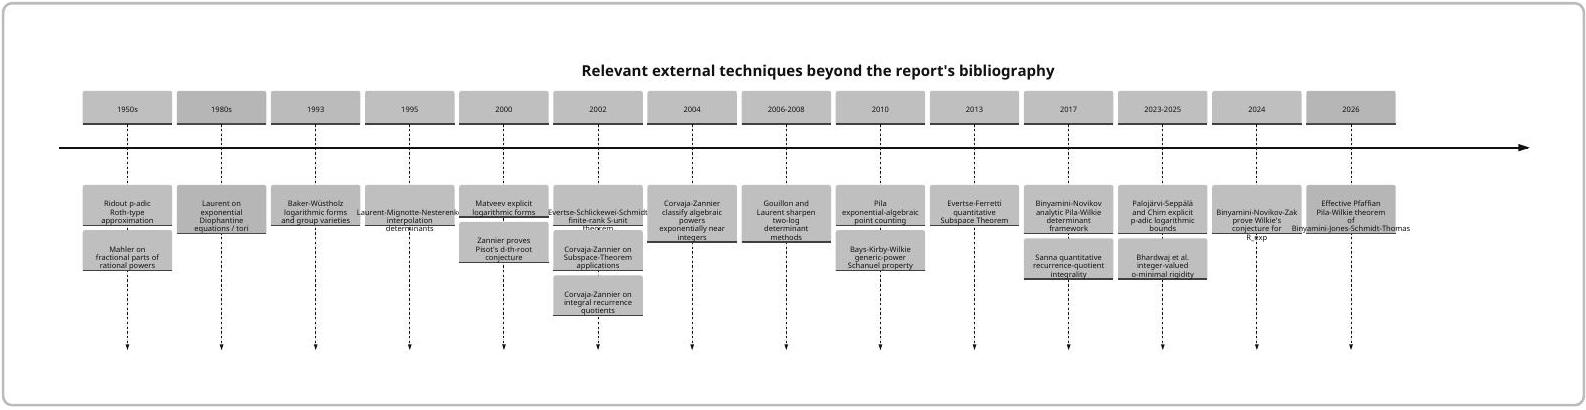
\includegraphics[max width=\textwidth, alt={}, center]{14655053-5393-4a14-bc7a-9901afeb0814-11_410_1586_446_269}

\section*{Proof strategies worth trying}
The rank-two-group/Pfaffian strategy should become a first-class program.

The proposed target


\begin{equation*}
N_{\Gamma}(T)=\#\{P \in \Gamma \cap \mathcal{C}: h(P) \leq T\}=o(T) \tag{6}
\end{equation*}


encapsulates the exact contradiction needed. It is materially narrower than the four-exponentials conjecture: the group is generated by two rational points, the analytic curve is the single fixed curve $v=$ $u^{\log _{2} 3}$, all points lie in a compact rectangle, and the relevant orbit is not all of $\Gamma$ but the diagonal/ synchronized sequence (2).

A useful attack on (6) would have two stages.

Construct, from a block of $N$ orbit points, a sparse Laurent polynomial

$$
F(X, Y)=\sum_{j=1}^{s} c_{j} X^{a_{j}} Y^{b_{j}}
$$

vanishing on many of them. The polynomial need not have small total degree; what matters for the $S$-unit stage is a small number $s$ of monomials. This distinction is essential. Classical interpolation determinants are particularly well suited to controlling support rather than merely total degree. Laurent-Mignotte-Nesterenko provide the natural model. ${ }^{11}$

Then apply finite-rank multiplicative-group theory to $F(P)=0$. Each monomial $P \mapsto P_{1}^{a_{j}} P_{2}^{b_{j}}$ stays in a group of rank at most two. Evertse-Schlickewei-Schmidt therefore bounds nondegenerate solutions once $s$ is fixed. 6 Degenerate subsums reduce support and can be handled recursively; two-term terminal equations are torus cosets, which meet $\mathcal{C}$ in at most one real point.

The resulting technical target is sharper than "improve Pila-Wilkie":

Cover the synchronized orbit up to height $T$ by $o(T)$ Laurent curves of uniformly bounded $\sup (p) \mathrm{rt}$.\\
This would immediately expose the orbit to $S$-unit rigidity. The degree of those Laurent polynomials may be allowed to grow substantially if the support remains bounded.

A variant replaces exact vanishing by determinants. Take monomial columns $X^{a_{j}} Y^{b_{j}}$ and rows $P_{k_{i}}$. If enough arithmetic divisibility makes the determinant's lower bound exceed its archimedean upper bound unless the determinant vanishes, one has precisely generated the algebraic covering required by (7). This unifies the report's determinant priorities A-C rather than treating determinant and o-minimal counting as separate projects.

\section*{The determinant should be optimized in the Laurent/LMN design space.}
The report's generalized Vandermonde construction uses positive monomials and gains nonvanishing/ integrality almost for free. The price is that its dimension/weight balance misses the hypothetical population by one $\log X$. Laurent's interpolation-determinant machinery suggests four concrete changes.

Use confluent multiplicities rather than one evaluation condition per node. The report already notices finite differences as confluent determinants. LMN-style multiplicity allocation is the systematic version of this observation. ${ }^{2}$

Use asymmetric support regions in $(a, b)$-space. The natural columns need not be the first $r$ monomials ordered by $a+\theta b$. One should optimize a convex/lattice region against both archimedean weight and known 2- and 3-adic valuation forms.

Introduce zero-lemma constraints into the search. It is often cheaper to prove that an auxiliary function cannot vanish to specified multiplicities unless a forbidden algebraic relation occurs than to establish positivity of a very large generalized Vandermonde.

Finally, permit integer-preserving basis changes among columns. Falling-factorial, binomial, and finite-difference bases can have radically better local divisibility than ordinary powers while generating the same polynomial module. Because unimodular column transformations preserve determinant up to sign, this is potentially "free" arithmetic gain.

The computational optimization problem should therefore stop being

$$
\text { choose monomials minimizing } \sum(a+\theta b)
$$

and become approximately


\begin{equation*}
\max _{\mathcal{R}, \mathcal{E}, \mathcal{T}}\left[L_{2} \log 2+L_{3} \log 3-U_{\infty}\right], \tag{8}
\end{equation*}


where $\mathcal{R}$ is a selected region of row coordinates $(n, k), \mathcal{E}$ a sparse exponent set $(a, b), \mathcal{T}$ a unimodular/ difference transformation, $L_{p}$ is a proven lower bound for the determinant's $p$-adic valuation, and $U_{\infty}$ is a rigorous archimedean upper bound.

\section*{Use tropical determinant valuations before invoking $p$-adic logarithms.}
For the raw monomial entry

$$
E_{i j}=\left(2^{n_{i}} M^{k_{i}}\right)^{a_{j}}\left(3^{n_{i}} A^{k_{i}}\right)^{b_{j}},
$$

the 2- and 3-adic valuations are affine bilinear forms in the row and column parameters. This makes the valuation of each permutation term in the determinant exactly computable. The guaranteed common $p$ power dividing the determinant is bounded below by the min-plus determinant


\begin{equation*}
L_{p}=\min _{\sigma} \sum_{i} v_{p}\left(E_{i, \sigma(i)}\right) . \tag{9}
\end{equation*}


The report correctly finds that the raw presence of the $(0,0)$ monomial often destroys the gain. That should motivate transforming the basis before computing (9), not abandoning the min-plus approach.

Finite differences along a lattice direction ( $\Delta n, \Delta k$ ) transform a monomial sequence by factors related to


\begin{equation*}
R_{a, b}=2^{a \Delta n} 3^{b \Delta n} M^{a \Delta k} A^{b \Delta k}-1 . \tag{10}
\end{equation*}


Such factors can acquire nontrivial $p$-adic valuations. One should search for directions for which these valuations grow faster than the corresponding archimedean cost. This is a natural location for lifting-theexponent arguments, multiplicative-order calculations modulo $p^{s}$, and eventually explicit $p$-adic logarithmic forms.

Chim's theorem is especially useful in the cancellation stage. It gives explicit upper bounds for

$$
v_{p}\left(\alpha_{1}^{b_{1}}-\alpha_{2}^{b_{2}}\right)
$$

for algebraic $\alpha_{i}$, with favorable $\log B$ dependence. ${ }^{13}$ Thus if a tropical argument identifies a small set of permutation terms of minimal valuation, Chim-type bounds can control how much their normalized $p$-adicunit sum can cancel. Palojärvi-Seppälä offer another explicit rational/algebraic $p$-adic framework, while Gaudron is relevant if one can formulate the determinant globally over several places. ${ }^{31}$

A particularly attractive endgame would be a product-formula contradiction

$$
0 / D \fallingdotseq \mathbf{Z}, \quad \log |D|_{\infty}+\sum_{p} \log |D|_{p}=0,
$$

where the archimedean determinant estimate is negative enough after the $p=2,3$ gains. This is conceptually stronger than merely replacing $1 \leq|D|$ with $2^{L_{2}} 3^{L_{3}} \leq|D|$.

\section*{Search explicitly for a recurrence quotient.}
Corvaja-Zannier's recurrence theorem should be treated as a challenge to construct an object of the right form, not as an immediately applicable result.

Along an affine line in the conditional $(n, k)$-grid,

$$
(n, k)=\left(n_{0}, k_{0}\right)+t(r, s),
$$

any monomial in the two outputs becomes a geometric sequence in $t$. A finite linear combination is therefore a power sum/linear recurrence. Determinant minors, finite differences and interpolation coefficients restricted to such a line are consequently ratios of power sums surprisingly often.

The concrete search is:

$$
Q(t)=\frac{F(t)}{G(t)},
$$

where $F, G$ are low-complexity power sums derived canonically from candidate points, and prove from the integrality of the original points that $Q(t) \in \mathbf{Z}$ for infinitely many $t$. If this succeeds, Corvaja-Zannier force $Q$, after controlled modifications and an arithmetic progression, back into recurrence structure. ${ }^{30}$ Sanna then gives quantitative density constraints where the quotient is genuinely nontrivial. ${ }^{26}$

Promising sources for $Q(t)$ are ratios of adjacent determinant minors, Newton interpolation coefficients, divided differences after clearing the canonical Vandermonde denominator, and Smith-normal-form invariant factors of evaluation matrices. These are preferable to arbitrary rational functions because integrality/divisibility may follow automatically from the integer matrix structure already formalized in the report.

\section*{Try to manufacture a Mahler-Pisot contradiction.}
Corvaja-Zannier's 2004 theorem is exceptionally clean as an endgame. If $\alpha>1$ is algebraic and is not a $d$ th root of a Pisot number, then its powers cannot be exponentially close to integers infinitely often in the forbidden way; this solves Mahler's old question by Subspace-Theorem methods. ${ }^{16}$

Consequently the following intermediate lemma would settle AE:

From a nonintegral $\beta$ with $2^{\beta}, 3^{\beta} \in \mathbf{Z}$, construct a fixed algebraic $\alpha>1$, not a root of a Pisot number, a fixed $0<\lambda<1$, and infinitely many $n$ satisfying

$$
>\left\|\alpha^{n}\right\|<\lambda^{n} .>
$$

The most obvious candidates are rational normalizations

$$
\alpha=\frac{M}{2^{r}}, \quad \alpha^{\prime}=\frac{A}{3^{s}},
$$

or algebraic expressions from the report's radical field. For rational $\alpha$, the exceptional Pisot-root alternative is very restrictive: if a rational number has an integral power that is an algebraic integer, valuation considerations force strong integrality constraints. The difficult part is producing the exponential nearness from the simultaneous base-2/base-3 synchronization.

This deserves computational exploration because it has an unusually binary outcome: either the synchronized dynamics exhibits an unexpectedly strong near-integer phenomenon, in which case one has a powerful theorem ready to use, or experiments quickly show that this family of bridges is implausible.

Use explicit logarithmic forms where they are actually strongest.

Matveev and Baker-Wüstholz should not be pointed at (1). They should be deployed on relations created by auxiliary constructions. ${ }^{32}$ For example,

$$
|q \log M-p \log 2|, \quad|q \log A-p \log 3|, \quad|a \log M+b \log A+c \log 2+d \log 3|,
$$

are legitimate targets.

For two logarithms, Gouillon's specialized constants can be much better than generic Matveev. ${ }^{23}$ Laurent's interpolation determinant can be better still in carefully tuned situations. If a third independent algebraic exponential is manufactured, Mignotte-Voutier's three-log toolkit becomes the computationally natural next step. ${ }^{24}$

Their expected payoff is an effective exclusion theorem of the form

$$
M \leq B \quad \Longrightarrow \quad \text { no counterexample },
$$

with $B$ many orders of magnitude beyond brute-force interval search, or a rigorous uniform certificate that eliminates a family of valuation/radical configurations. They are unlikely, by themselves, to turn the exponentially weak rational-approximation contradiction analyzed in the report into a global proof.

\section*{Model theory, recurrence theory, and where the tempting approaches stop}
The model-theoretic literature gives both useful structure and a warning.

Bays, Kirby and Wilkie prove a Schanuel property for power maps with an exponentially transcendental exponent; later work on generic powers builds on that fact, and only countably many complex exponents are outside the exponentially-transcendental class. ${ }^{5}$ It would therefore be natural to hope that $\theta=$ $\log _{2} 3$ is covered by a generic theorem.

It is not. This can be checked directly. Consider the exponential-polynomial system

$$
f_{1}(z, w)=e^{z}-2, \quad f_{2}(z, w)=e^{z w}-3 .
$$

At

$$
(z, w)=\left(\log 2, \frac{\log 3}{\log 2}\right)
$$

both vanish, and

$$
\operatorname{det}\left(\begin{array}{cc}
e^{z} & 0 \\
w e^{z w} & z e^{z w}
\end{array}\right)=6 \log 2 / 0 .=
$$

Thus $\theta$ belongs to the exponential algebraic closure in the Khovanskii-system sense. This is an inference from the definition used in the generic-power literature: the Alaoglu-Erdős exponent parameter falls precisely into the exceptional countable set to which the generic Schanuel-property theorem does not apply. ${ }^{5}$

This also helps explain why Schanuel itself is so much stronger here. The attached report already observes that Schanuel implies the required prime-log-product independence. Nothing in the newer generic-power literature seems to weaken that conditional assumption specifically at the exceptional value $\log _{2} 3$.

Zilber-Pink and anomalous-intersection theory are likewise one step removed. Bombieri-Masser-Zannier's theory concerns intersections of algebraic subvarieties of tori with algebraic subgroups and their atypical components. ${ }^{27}$ The relevant AE curve $v=u^{\theta}$ is transcendental, even though the points on it are rational and belong to a finite-rank subgroup. Thus the useful order is\\
\textbackslash text\{transcendental arc\} \};\textbackslash xrightarrow\{ไtext\{determinant / o-minimal covering\}\}; \textbackslash text\{algebraic curves\} ; \textbackslash xrightarrow\{\textbackslash text\{KATEX157-unit / toric theory\}\}; \textbackslash text\{finiteness\},\\
rather than applying Zilber-Pink directly. A 2026 survey by Capuano gives an up-to-date account of the toric Zilber-Pink landscape and its relationship with Schanuel-type questions, but for AE it is best viewed as background for the second arrow. ${ }^{29}$

Skolem-Mahler-Lech has a similar limitation. Its natural domain is the zero set of a fixed linear recurrence or, in modern dynamical forms, the intersection times of an algebraic orbit with an algebraic subvariety. The unnormalized sequence

$$
\left(M^{k}, A^{k}\right)
$$

is certainly an algebraic dynamical orbit, but the condition connecting its coordinates,

$$
\log \left(A^{k}\right) / \log 3=\log \left(M^{k}\right) / \log 2,
$$

is transcendental rather than algebraic. The normalization by $\lfloor k \beta\rfloor$ makes the points compact but introduces the floor operation. Hence Skolem-Mahler-Lech becomes powerful after one has created an auxiliary algebraic relation or recurrence zero, not before.

Zannier's proof of Pisot's $d$-th-root conjecture is instructive in exactly this way. If the coefficients of a rational generating function are eventually perfect $d$-th powers, one can choose their roots so that the resulting generating series is rational as well. ${ }^{25}$ That is an extraordinarily rigid conclusion from infinitely many perfect-power events. But the trivial sequence $M^{k}$ already has obvious perfect-power subsequences, so simply observing powers in the conditional monoid gains nothing. One needs a less tautological recurrence-preferably a determinant minor or quotient generated simultaneously by the 2- and 3-coordinates.

The same caveat applies to contemporary multiplicative-dependence results. Young's 2024 work classifies situations in polynomial dynamics with infinitely many multiplicative-dependence relations and proves\\
sparsity results for index vectors in broad classes. ${ }^{28}$ This reinforces a common theme-persistent multiplicative dependence generally signals special algebraic structure-but the AE semigroup is already deliberately rank two. A theorem saying "the rank is small" cannot collapse rank two to rank one; the report has correctly identified that as the heart of the conjecture.

There are also useful counterexamples to naive proof heuristics.

A single base is hopeless: for every integer $m>1$,

$$
x=\log _{2} m
$$

makes $2^{x}=m$ an integer, and $x$ is usually nonintegral.

Multiplicative independence of the bases is essential. For 2 and 4, every $x=\log _{2} m$ gives both $2^{x}=m$ and $4^{x}=m^{2}$ integral.

Metric equidistribution cannot rule out exponentially shrinking targets: the report's diagnosis is consistent with standard Diophantine dynamics. The special information must come from the arithmetic relation between the two bases.

Nor can one assume that "algebraic powers cannot approach integers exponentially." Pisot numbers are exactly a celebrated family whose powers do so, and Corvaja-Zannier's theorem has to retain Pisot-root exceptions. ${ }^{33}$ Any Mahler-style route therefore needs to identify and exclude its exceptional algebraic bases rather than argue from generic behavior.

Finally, general o-minimal point counting is quantitatively too permissive. The 2024 Wilkie theorem gives polylogarithmic growth in multiplicative height, not a universal $o(\log H)$ bound. 7 The new 2026 effective theorem makes constants and complexity effective but does not by itself change this fundamental exponent issue. 8 Thus the report is correct that denominator support, finite multiplicative rank, or synchronization must be brought into the count.

\section*{Computational experiments and concrete next steps}
The computational program should be aimed less at increasing the numerical zero-free bound and more at discovering the missing arithmetic inequality. The report's existing formalized structure makes several experiments unusually well posed.

Build a tropical/interpolation determinant optimizer. Represent a row by $\left(n_{i}, k_{i}\right)$, a column by $\left(a_{j}, b_{j}\right)$, and record symbolically

$$
\begin{aligned}
& v_{2}\left(E_{i j}\right)=a_{j}\left(n_{i}+v_{2}(M) k_{i}\right)+b_{j} v_{2}(A) k_{i}, \\
& v_{3}\left(E_{i j}\right)=a_{j} v_{3}(M) k_{i}+b_{j}\left(n_{i}+v_{3}(A) k_{i}\right) .
\end{aligned}
$$

For each candidate row/column shape compute the tropical determinant lower bounds $L_{2}, L_{3}$, then a certified archimedean determinant bound. Search the objective (8), not merely the archimedean exponent.

The search space should include triangular regions

$$
n+k \beta \leq T,
$$

rectangular $(n, k)$-blocks, skew parallelograms aligned to convergents of $\beta$, and sparse exponent supports aligned to the dual weight $a+\theta b$. Treat $v_{2}(M), v_{3}(M), v_{2}(A), v_{3}(A)$ symbolically where possible, using the primitive-output constraints already proved in the report.

Search over unimodular column bases. For each monomial support, generate transforms based on falling factorials and finite differences. A difference along a vector $(r, s)$ naturally introduces factors of the form

$$
2^{a r} 3^{b r} M^{a s} A^{b s}-1 .
$$

Compute exact 2- and 3-adic valuations of these factors and their archimedean sizes. Search for repeated difference directions that yield a positive asymptotic valuation/size ratio. The determinant is unchanged up to a unit under appropriate integer basis transformations, so a successful basis is immediately theoremshaped rather than merely numerical.

Perform a min-plus cancellation study. When several determinant permutations attain the same minimal $p$-adic valuation, divide out the forced factor and study the remaining $p$-adic unit sum. Classify cases in which it reduces to a two-term difference of powers. Those are direct candidates for Chim's 2025 theorem.\\
${ }^{13}$ Cases involving more terms should be catalogued against available $S$-unit and $p$-adic-log bounds rather than treated generically.

The output of this experiment should not just be "large valuation observed." It should emit a certificate containing the row set, column support, integer basis transformation, forced $p$-power, tropical assignment proof, and archimedean bound. That makes successful examples easy to port into Lean.

Search for sparse Laurent relations rather than low-degree polynomials. Given blocks of near-counterexample numerical data, solve for Laurent polynomials with the smallest support cardinality that nearly vanish on the normalized arc points. Penalize monomial count much more heavily than degree. The goal is to discover supports for which an interpolation determinant might be forced to vanish arithmetically.

The reason is the ESS theorem: an $s$-term relation on a rank-two multiplicative group is the natural $S$-unit unit of complexity. ${ }^{6}$ A degree-1000 binomial can be more useful than a dense degree-10 polynomial.

Because no actual counterexample $M, A$ is known, use near-counterexamples. For integers $M$ in a large range set

$$
A=\operatorname{round}\left(M^{\theta}\right), \quad \delta(M)=\log M \log 3-\log A \log 2 .
$$

Rank values by $|\delta(M)|$, then investigate whether the unusually small residuals correlate with determinant valuations, sparse relations, or recurrence quotients. This does not prove anything about exact zeros, but it is a useful adversarial test for candidate inequalities: any proposed proof mechanism should be stresstested against the best finite approximants to the forbidden bilinear relation.

Automate the recurrence-quotient search. Along many affine directions

$$
(n, k)=\left(n_{0}, k_{0}\right)+t(r, s),
$$

construct low-order minors of the evaluation matrix, Newton coefficients, divided differences, and Smith invariant factors. Symbolically express each as a quotient of power sums in $t$. Test whether candidate integrality/divisibility follows identically from the integer inputs. Any nontrivial quotient that is forced integral on infinitely many $t$ should immediately be compared with Corvaja-Zannier and Sanna. ${ }^{34}$

A very useful automated filter would reject quotients that simplify to a trivial monomial/geometric sequence. The interesting outputs are exactly those whose integrality is nonobvious but follows from a determinant identity.

Search for a Mahler-Pisot bridge. For near-counterexamples $M, A$, enumerate modest-height rational/ algebraic expressions

$$
\alpha=M^{a} A^{b} 2^{c} 3^{d}
$$

and radical-field expressions suggested by the report. Compute

$$
-\frac{1}{n} \log \left\|\alpha^{n}\right\|
$$

over sizable ranges of $n$. A genuine positive limsup bounded away from zero is the numerical fingerprint of exponential closeness needed for the Corvaja-Zannier theorem. ${ }^{33}$ Expressions showing merely polynomially good approximation should be discarded.

This experiment is especially worthwhile because the theory already tells us exactly what a successful signal means: either $\alpha$ belongs to the Pisot-root exceptional class or a hypothetical counterexample is impossible.

Upgrade finite verification with specialized logarithmic-form certificates. The report's interval computations can be supplemented by two-log bounds specialized to

$$
q \log M-p \log 2
$$

rather than generic high-dimensional Baker estimates. Laurent's 2008 determinant bounds and Gouillon's explicit results are the first places to look. ${ }^{35}$ Matveev provides a robust fallback for auxiliary forms with more logarithms. ${ }^{22}$ For three-log forms arising after an auxiliary-base construction, Mignotte-Voutier's framework is designed for actual computation rather than just asymptotic existence. ${ }^{24}$

The objective should be a machine-checkable theorem schema

$$
\text { parameter inequalities ⟹ }|\Lambda|>\text { explicit threshold } \text { ⟹ candidate impossible, }
$$

rather than a large table of independently evaluated transcendental numbers.

Formulate and attack one new theorem at a time. The following order appears optimal.

The first theorem to target is the sparse-cover statement (7). Even a conditional or weak quantitative result would reveal whether the $S$-unit hybrid is viable.

In parallel, rebuild one of the report's semigroup determinants in Laurent-style confluent form and optimize it computationally. The goal is to determine whether multiplicities can reduce the node requirement from $O\left((\log X)^{2}\right)$ toward $O(\log X)$.

Next, add 2- and 3-adic valuation objectives to that same determinant rather than developing a wholly separate $p$-adic argument.

Only after these experiments should substantial effort go into general Zilber-Pink or Skolem-Mahler-Lech formalization. Those theories become relevant if the preceding stages produce an algebraic curve or recurrence; without such a bridge they do not touch the transcendental relation.

The resulting research dependency graph is:\\
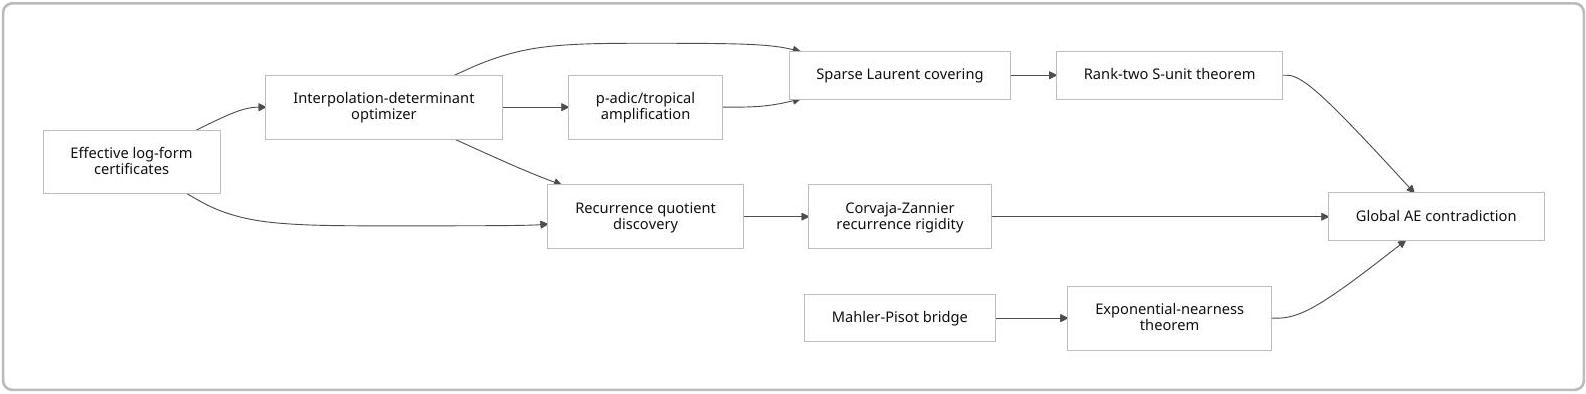
\includegraphics[max width=\textwidth, alt={}, center]{14655053-5393-4a14-bc7a-9901afeb0814-20_394_1586_882_269}

The strategically important point is that these branches do not all require solving a new transcendence theorem comparable with four exponentials. The sparse-cover/ $S$-unit branch asks whether the very special infinite family forced by a counterexample is too arithmetic to inhabit the exponential arc. That is a more structured question than arbitrary four exponentials and appears to be the best place to exploit the report's exact conditional classification.

\section*{Gaps that remain and the most useful research questions}
The literature survey sharpens the remaining barrier into a small number of explicit open subproblems.

There is no known lower bound for the prime-log-product form required directly by the report. The relation

$$
\sum_{p}\left(m_{p} \log 3-a_{p} \log 2\right) \log p=0
$$

has logarithmic, hence transcendental, coefficients. Matveev, Baker-Wüstholz, Gouillon and the modern $p$ adic analogues all concern linear forms in logarithms with integer/algebraic coefficients; none turns this bilinear form into an admissible Baker form. ${ }^{36}$ Thus importing stronger constants into Baker's method cannot by itself solve the problem.

The exact missing counting theorem is below the present general o-minimal threshold. Binyamini-Novikov-Zak give a power of $\log H$ for rational points on transcendental Pfaffian sets. 7 A counterexample only yields order $\log H$ points. The 2026 effective theorem provides extraordinarily useful\\
uniformity but still does not automatically force an exponent < 1. 8 The gap is therefore not "make Pila-Wilkie effective"; it is "incorporate fixed multiplicative rank and synchronized prime support strongly enough to save a power of logarithmic height."

No bridge to the Subspace Theorem has yet been identified. The Subspace Theorem is devastating once one obtains a sufficiently good algebraic approximation or $S$-unit equation. Evertse-Ferretti improve its quantitative form, and Corvaja-Zannier demonstrate how to turn integrality of power-series/power-sum values into precisely such inequalities. ${ }^{37}$ The AE condition itself remains logarithmic rather than algebraic. The research problem is to make a determinant, finite difference, radical norm, or interpolation coefficient produce a genuine Subspace-Theorem inequality.

The recurrence literature is waiting for the right auxiliary sequence. Corvaja-Zannier, Zannier's root theorem, and Sanna become powerful only after an infinite sequence of perfect-power, integral-quotient, or small-value events is produced. ${ }^{38}$ The existing conditional monoid gives many trivial recurrences, but none yet combines the two bases in a nontrivial integral quotient.

The Mahler/Pisot route has a beautifully sharp missing lemma. Corvaja-Zannier have already done the difficult Diophantine approximation once an algebraic number has powers exponentially close to integers.\\
${ }^{33}$ The missing question is whether simultaneous 2- and 3-integrality forces any fixed algebraic normalization into that situation.

The $p$-adic determinant direction needs a mechanism for forced divisibility, not merely stronger logarithmic-form estimates. Chim's theorem bounds how deeply differences of algebraic powers can vanish $p$-adically. ${ }^{13}$ To exploit it, one first needs a determinant basis in which a substantial common 2- or 3 -power is forced by combinatorics of valuations. The natural mathematical objects here are tropical determinants, finite-difference bases, multiplicative orders, and possibly confluent interpolation determinants.

Generic model theory provably misses the relevant parameter. The inference above that $\log _{2} 3$ is exponentially algebraic means that the generic-power Schanuel theorem of Bays-Kirby-Wilkie is not a shortcut. 5 Any model-theoretic progress would need to exploit the structure of this exceptional exponential-algebraic parameter, which is essentially where Schanuel/four-exponentials difficulty resides.

The strongest new "research questions" I would add to the internal report are therefore:

\footnotetext{\textbackslash boxed\{ \textbackslash begin\{minipage\}\{0.88\textbackslash linewidth\} Can a rank-two subgroup of KATEX219 meet the specific arc
} KATEX220 in KATEX221 synchronized KATEX222-integral points of logarithmic height at most KATEX223?\\
\textbackslash end\{minipage\}\} \}\\
\textbackslash boxed\{ \textbackslash begin\{minipage\}\{0.88\textbackslash linewidth\} Can the conditional orbit be covered, up to logarithmic height \} KATEX224, by KATEX225 Laurent curves having uniformly bounded numbers of monomials?\\
\textbackslash end\{minipage\}\} \}\\
\textbackslash boxed\{ \textbackslash begin\{minipage\}\{0.88\textbackslash linewidth\} Is there a unimodular/confluent basis of the semigroup \} evaluation determinant for which the KATEX226- and KATEX227-adic tropical determinant contributes KATEX228 while the archimedean cost is KATEX229? lend\{minipage\} \}\\
\textbackslash boxed\{ \textbackslash begin\{minipage\}\{0.88\textbackslash linewidth\} Can one construct from the synchronized KATEX230-/KATEX231- \}orbit a nontrivial quotient of power sums that is integral infinitely often? \textbackslash end\{minipage\} \} \}\\
\}\\
\textbackslash boxed\{ \textbackslash begin\{minipage\}\{0.88\textbackslash linewidth\} Can one construct a fixed non-Pisot algebraic KATEX232 whose \} powers are exponentially close to integers as a consequence of a counterexample? \textbackslash end\{minipage\} \} \}

Each question has an existing major theorem on the other side of the missing bridge. That is a much better situation than attempting directly to prove a new lower bound for arbitrary products of logarithms.

\section*{Selected bibliography and source links}
The following is the bibliography I would add first to the internal report. The ordering reflects usefulness to this specific problem rather than historical priority.\\
J.-H. Evertse, H. P. Schlickewei, W. M. Schmidt, "Linear equations in variables which lie in a multiplicative group," Annals of Mathematics 155 (2002), 807-836, DOI 10.2307/3062133. Gives a quantitative bound for nondegenerate solutions of linear equations in finite-rank multiplicative groups. Annals source. ${ }^{6}$\\
M. Laurent, M. Mignotte, Yu. Nesterenko, "Formes linéaires en deux logarithmes et déterminants d'interpolation," Journal of Number Theory 55 (1995), 285-321, DOI 10.1006/jnth.1995.1141. Introduces the interpolation-determinant/zero-lemma architecture that is especially relevant to the report's determinant deficit. Publisher record. ${ }^{11}$\\
M. Laurent, "Linear forms in two logarithms and interpolation determinants II," Acta Arithmetica 133 (2008), 325-348, DOI 10.4064/aa133-4-3. IMPAN article page. ${ }^{12}$\\
K. C. Chim, "Lower bounds for linear forms in two $p$-adic logarithms," Journal of Number Theory 266 (2025), 295-349, DOI 10.1016/j.jnt.2024.07.012. Gives explicit bounds for $v_{p}\left(\alpha_{1}^{b_{1}}-\alpha_{2}^{b_{2}}\right)$ with $\log B$ dependence in the two-log setting. Publisher article. ${ }^{13}$\\
G. Binyamini, D. Novikov, B. Zak, "Wilkie's conjecture for Pfaffian structures," Annals of Mathematics 199 (2024), 795-821, DOI 10.4007/annals.2024.199.2.5. Proves effective polylogarithmic rational-point counting for restricted sub-Pfaffian structures and, as a corollary, Wilkie's conjecture for $\mathbb{R}_{\text {exp }}$. Annals source. 7\\
G. Binyamini, G. Jones, H. Schmidt, M. E. M. Thomas, "An effective Pila-Wilkie theorem for sets definable using Pfaffian functions, with some diophantine applications," Journal of the European Mathematical Society, online first 2026, DOI 10.4171/JEMS/1761. Published April 15, 2026. EMS article. ${ }^{8}$\\
P. Corvaja, U. Zannier, "Some New Applications of the Subspace Theorem," Compositio Mathematica 131 (2002), 319-340, DOI 10.1023/A:1015594913393. Applies the Subspace Theorem to $S$-unit arguments, Laurent-series values, power sums and Mahler-type transcendence problems. Cambridge record. ${ }^{14}$\\
P. Corvaja, U. Zannier, "Finiteness of integral values for the ratio of two linear recurrences," Inventiones Mathematicae 149 (2002), 431-451, DOI 10.1007/s002220200221. If a ratio of recurrences is integral infinitely often, derives strong recurrence structure after controlled modifications. ${ }^{15}$\\
P. Corvaja, U. Zannier, "On the rational approximations to the powers of an algebraic number: solution of two problems of Mahler and Mendès France," Acta Mathematica 193 (2004), 175-191, DOI 10.1007/

BF02392563. Classifies exponential approximation of algebraic powers to integers, with Pisot-root exceptions. arXiv version. ${ }^{16}$\\
N. Bhardwaj, R. McCulloch, N. Ramachandran, K. Woo, "Integer-valued o-minimal functions," Quarterly Journal of Mathematics 76 (2025), 715-729, DOI 10.1093/qmath/haaf027. Establishes strong rigidity for integer-valued $\mathbb{R}_{\text {an,exp }}$-definable functions under growth/concordance hypotheses. Oxford Academic.\\
J.-H. Evertse, R. G. Ferretti, "A further improvement of the Quantitative Subspace Theorem," Annals of Mathematics 177 (2013), 513-590, DOI 10.4007/annals.2013.177.2.4. Includes improved quantitative subspace bounds and refined information about height intervals. Annals source.\\
E. M. Matveev, "An explicit lower bound for a homogeneous rational linear form in the logarithms of algebraic numbers. II," Izvestiya: Mathematics 64 (2000), 1217-1269, DOI 10.1070/\\
IM2000v064n06ABEH000314. Standard explicit high-dimensional logarithmic-form estimate. MathNet.\\
A. Baker, G. Wüstholz, "Logarithmic forms and group varieties," Journal für die reine und angewandte Mathematik 442 (1993), 19-62, DOI 10.1515/crll.1993.442.19. De Gruyter.\\
N. Gouillon, "Explicit lower bounds for linear forms in two logarithms," Journal de Théorie des Nombres de Bordeaux 18 (2006), 125-146, DOI 10.5802/jtnb.537. Particularly useful when a derived AE subproblem has exactly two logarithms. Centre Mersenne.\\
M. Mignotte, P. Voutier, "A kit for linear forms in three logarithms," arXiv:2205.08899; subsequently published in Mathematics of Computation, DOI 10.1090/mcom/3908. Gives an implementable specialized method and worked examples. arXiv.\\
N. Palojärvi, L. Seppälä, "A $p$-adic lower bound for a linear form in logarithms," International Journal of Number Theory 19 (2023), 261-291, DOI 10.1142/S1793042123500136. University of Helsinki record, with manuscript.

É. Gaudron, "Minorations simultanées de formes linéaires de logarithmes de nombres algébriques," arXiv: 1004.3652 (2010). Treats simultaneous archimedean and $p$-adic linear forms using adelic slope methods.\\
arXiv. ${ }^{20}$\\
U. Zannier, "A proof of Pisot's $d^{\text {th }}$ root conjecture," Annals of Mathematics 151 (2000), 375-383, DOI 10.2307/121122. A fundamental perfect-power rigidity theorem for recurrence/rational-generating-function coefficients. Annals.\\
C. Sanna, "Distribution of integral values for the ratio of two linear recurrences," Journal of Number Theory 180 (2017), 195-207, DOI 10.1016/j.jnt.2017.04.015. Gives quantitative density bounds refining the Corvaja-Zannier setting. Publisher record.\\
J. Pila, "Counting rational points on a certain exponential-algebraic surface," Annales de l'Institut Fourier 60 (2010), 489-514, DOI 10.5802/aif.2530; correction, AIF 67 (2017), 1277-1278, DOI 10.5802/aif.3109. A specialized exponential-algebraic counting theorem closer to AE than the generic Pila-Wilkie statement. Original; correction.\\
G. Binyamini, D. Novikov, "The Pila-Wilkie theorem for subanalytic families: a complex analytic approach," Compositio Mathematica (2017). Recasts rational-point counting through complex analysis and interpolation determinants, making it especially relevant to merging the report's determinant and counting programs.\\
10\\
M. Bays, J. Kirby, A. J. Wilkie, "A Schanuel property for exponentially transcendental powers," Bulletin of the London Mathematical Society 42 (2010), 917-922, DOI 10.1112/blms/bdq054. Valuable mainly for identifying exactly why generic-power model theory does not encompass $\log _{2} 3$. ${ }^{5}$\\
E. Bombieri, D. Masser, U. Zannier, "Anomalous Subvarieties-Structure Theorems and Applications," International Mathematics Research Notices 2007, rnm057, DOI 10.1093/imrn/rnm057. Relevant after an interpolation step has converted the transcendental arc into algebraic toric intersection problems. Oxford Academic. ${ }^{27}$\\
M. Laurent, "Équations diophantiennes exponentielles," Séminaire de Théorie des Nombres de Bordeaux (1983-84). A useful classical entry point to exponential Diophantine equations and intersections with algebraic tori. EuDML. ${ }^{39}$\\
M. Young, "On multiplicative dependence between elements of polynomial orbits," arXiv:2402.13712 (2024). Illustrates modern structural/sparsity results for persistent multiplicative dependence. arXiv. ${ }^{28}$\\
L. Capuano, "Exploring Zilber's conjecture on atypical intersections in tori and beyond," Journal of the London Mathematical Society (2026), DOI 10.1112/jlms.70536. A current survey of the unlikely-intersection landscape and links to Schanuel-type questions. ${ }^{29}$

The literature therefore does not reveal a missed theorem that simply resolves Alaoglu-Erdős. It does reveal something more actionable: the attached report's remaining barrier sits at the intersection of several mature theories that have not yet been combined in its current form. The most promising synthesis is to use the exact rank-two conditional subgroup and synchronized denominators to strengthen an interpolation/o-minimal count, then hand the resulting sparse algebraic relations to $\boldsymbol{S}$-unit theory. In parallel, Laurent-style interpolation determinants and tropical $p$-adic amplification provide the most technically direct way to attack the report's precisely quantified one- $\log X$ determinant deficit.

\footnotetext{16 \href{https://annals.math.princeton.edu/2002/155-3/p04}{https://annals.math.princeton.edu/2002/155-3/p04}\\
\href{https://annals.math.princeton.edu/2002/155-3/p04}{https://annals.math.princeton.edu/2002/155-3/p04}\\
211 \href{https://www.sciencedirect.com/science/article/pii/S0022314X85711419}{https://www.sciencedirect.com/science/article/pii/S0022314X85711419}\\
\href{https://www.sciencedirect.com/science/article/pii/S0022314X85711419}{https://www.sciencedirect.com/science/article/pii/S0022314X85711419}\\
${ }^{3} 13$ \href{https://www.sciencedirect.com/science/article/pii/S0022314X24001793}{https://www.sciencedirect.com/science/article/pii/S0022314X24001793}\\
\href{https://www.sciencedirect.com/science/article/pii/S0022314X24001793}{https://www.sciencedirect.com/science/article/pii/S0022314X24001793}\\
4153034 \href{https://www.researchgate.net/publication/}{https://www.researchgate.net/publication/}\\
226662209\_Finiteness\_of\_integral\_values\_for\_the\_ratio\_of\_two\_linear\_recurrences\\
\href{https://www.researchgate.net/publication/226662209_Finiteness_of_integral_values_for_the_ratio_of_two_linear_recurrences}{https://www.researchgate.net/publication/226662209\_Finiteness\_of\_integral\_values\_for\_the\_ratio\_of\_two\_linear\_recurrences}
}
\begin{itemize}
  \item[] ${ }^{5}$ \href{https://www.cambridge.org/core/journals/forum-of-mathematics-sigma/article/quasiminimality-of-complex-powers/344511AF0A83BA3313A160903826EA5A}{https://www.cambridge.org/core/journals/forum-of-mathematics-sigma/article/quasiminimality-of-complex-powers/344511AF0A83BA3313A160903826EA5A}\\
\href{https://www.cambridge.org/core/journals/forum-of-mathematics-sigma/article/quasiminimality-of-complex-powers/}{https://www.cambridge.org/core/journals/forum-of-mathematics-sigma/article/quasiminimality-of-complex-powers/} 344511AF0A83BA3313A160903826EA5A
  \item[7] \href{https://annals.math.princeton.edu/2024/199-2/p05}{https://annals.math.princeton.edu/2024/199-2/p05}\\
\href{https://annals.math.princeton.edu/2024/199-2/p05}{https://annals.math.princeton.edu/2024/199-2/p05}
  \item[8] \href{https://ems.press/journals/jems/articles/14299662}{https://ems.press/journals/jems/articles/14299662}\\
\href{https://ems.press/journals/jems/articles/14299662}{https://ems.press/journals/jems/articles/14299662}
  \item[] ${ }^{9}$ \href{https://numdam.org/articles/10.5802/aif.2530/}{https://numdam.org/articles/10.5802/aif.2530/}\\
\href{https://numdam.org/articles/10.5802/aif.2530/}{https://numdam.org/articles/10.5802/aif.2530/}
  \item[] ${ }^{10}$ \href{https://www.cambridge.org/core/journals/compositio-mathematica/article/pilawilkie-theorem-for-subanalytic-families-a-complex-analytic-approach/6BDD4C790E959BF2B94209AA9CF9BEBC}{https://www.cambridge.org/core/journals/compositio-mathematica/article/pilawilkie-theorem-for-subanalytic-families-a-complex-analytic-approach/6BDD4C790E959BF2B94209AA9CF9BEBC}\\
\href{https://www.cambridge.org/core/journals/compositio-mathematica/article/pilawilkie-theorem-for-subanalytic-families-a-complex-analytic-approach/6BDD4C790E959BF2B94209AA9CF9BEBC}{https://www.cambridge.org/core/journals/compositio-mathematica/article/pilawilkie-theorem-for-subanalytic-families-a-complex-analytic-approach/6BDD4C790E959BF2B94209AA9CF9BEBC}
  \item[1235] \href{https://www.impan.pl/en/publishing-house/journals-and-series/acta-arithmetica/all/133/4/82485/}{https://www.impan.pl/en/publishing-house/journals-and-series/acta-arithmetica/all/133/4/82485/} linear-forms-in-two-logarithms-and-interpolation-determinants-ii\\
\href{https://www.impan.pl/en/publishing-house/journals-and-series/acta-arithmetica/all/133/4/82485/linear-forms-in-two-logarithms-and-interpolation-determinants-ii}{https://www.impan.pl/en/publishing-house/journals-and-series/acta-arithmetica/all/133/4/82485/linear-forms-in-two-logarithms-and-interpolation-determinants-ii}
  \item[] ${ }^{14}$ \href{https://www.cambridge.org/core/journals/compositio-mathematica/article/some-new-applications-of-the-subspace-theorem/2F6BB76838F610EB90B204764335ABCA}{https://www.cambridge.org/core/journals/compositio-mathematica/article/some-new-applications-of-the-subspace-theorem/2F6BB76838F610EB90B204764335ABCA}\\
\href{https://www.cambridge.org/core/journals/compositio-mathematica/article/some-new-applications-of-the-subspace-theorem/}{https://www.cambridge.org/core/journals/compositio-mathematica/article/some-new-applications-of-the-subspace-theorem/} 2F6BB76838F610EB90B204764335ABCA
  \item[] ${ }^{16}{ }^{33}$ \href{https://arxiv.org/abs/math/0403522}{https://arxiv.org/abs/math/0403522}\\
\href{https://arxiv.org/abs/math/0403522}{https://arxiv.org/abs/math/0403522}
  \item[] ${ }^{17}$ \href{https://academic.oup.com/qjmath/advance-article/doi/10.1093/qmath/haaf027/8224436}{https://academic.oup.com/qjmath/advance-article/doi/10.1093/qmath/haaf027/8224436}\\
\href{https://academic.oup.com/qjmath/advance-article/doi/10.1093/qmath/haaf027/8224436}{https://academic.oup.com/qjmath/advance-article/doi/10.1093/qmath/haaf027/8224436}
  \item[1837] \href{https://annals.math.princeton.edu/2013/177-2/p04}{https://annals.math.princeton.edu/2013/177-2/p04}\\
\href{https://annals.math.princeton.edu/2013/177-2/p04}{https://annals.math.princeton.edu/2013/177-2/p04}
  \item[1931] \href{https://researchportal.helsinki.fi/en/publications/a-p-adic-lower-bound-for-a-linear-form-in-logarithms}{https://researchportal.helsinki.fi/en/publications/a-p-adic-lower-bound-for-a-linear-form-in-logarithms}\\
\href{https://researchportal.helsinki.fi/en/publications/a-p-adic-lower-bound-for-a-linear-form-in-logarithms}{https://researchportal.helsinki.fi/en/publications/a-p-adic-lower-bound-for-a-linear-form-in-logarithms}
  \item[] ${ }^{20}$ \href{https://arxiv.org/abs/1004.3652}{https://arxiv.org/abs/1004.3652}\\
\href{https://arxiv.org/abs/1004.3652}{https://arxiv.org/abs/1004.3652}
  \item[] ${ }^{21}$ \href{https://www.degruyterbrill.com/document/doi/10.1515/crll.1993.442.19/html}{https://www.degruyterbrill.com/document/doi/10.1515/crll.1993.442.19/html}\\
\href{https://www.degruyterbrill.com/document/doi/10.1515/crll.1993.442.19/html}{https://www.degruyterbrill.com/document/doi/10.1515/crll.1993.442.19/html}
  \item[223236] \href{https://www.mathnet.ru/eng/im314}{https://www.mathnet.ru/eng/im314}\\
\href{https://www.mathnet.ru/eng/im314}{https://www.mathnet.ru/eng/im314}
  \item[] ${ }^{23}$ \href{https://jtnb.centre-mersenne.org/articles/10.5802/jtnb.537/}{https://jtnb.centre-mersenne.org/articles/10.5802/jtnb.537/}\\
\href{https://jtnb.centre-mersenne.org/articles/10.5802/jtnb.537/}{https://jtnb.centre-mersenne.org/articles/10.5802/jtnb.537/}
  \item[] ${ }^{24}$ \href{https://arxiv.org/abs/2205.08899}{https://arxiv.org/abs/2205.08899}\\
\href{https://arxiv.org/abs/2205.08899}{https://arxiv.org/abs/2205.08899}
\end{itemize}

\\
\begin{itemize}
  \item[] ${ }^{25}{ }_{38}$ \href{https://annals.math.princeton.edu/2000/155-1/p13}{https://annals.math.princeton.edu/2000/155-1/p13}\\
\href{https://annals.math.princeton.edu/2000/155-1/p13}{https://annals.math.princeton.edu/2000/155-1/p13}
  \item[] ${ }^{26}$ \href{https://www.sciencedirect.com/science/article/pii/S0022314X17302019}{https://www.sciencedirect.com/science/article/pii/S0022314X17302019}\\
\href{https://www.sciencedirect.com/science/article/pii/S0022314X17302019}{https://www.sciencedirect.com/science/article/pii/S0022314X17302019}
  \item[] ${ }^{27}$ \href{https://academic.oup.com/imrn/article/674043}{https://academic.oup.com/imrn/article/674043}\\
\href{https://academic.oup.com/imrn/article/674043}{https://academic.oup.com/imrn/article/674043}
  \item[] ${ }^{28}$ \href{https://arxiv.org/abs/2402.13712}{https://arxiv.org/abs/2402.13712}\\
\href{https://arxiv.org/abs/2402.13712}{https://arxiv.org/abs/2402.13712}
  \item[] ${ }^{29}$ \href{https://londmathsoc.onlinelibrary.wiley.com/doi/full/10.1112/jlms}{https://londmathsoc.onlinelibrary.wiley.com/doi/full/10.1112/jlms}. 70536\\
\href{https://londmathsoc.onlinelibrary.wiley.com/doi/full/10.1112/jlms}{https://londmathsoc.onlinelibrary.wiley.com/doi/full/10.1112/jlms}. 70536
  \item[] ${ }^{39}$ \href{https://eudml.org/doc/182179}{https://eudml.org/doc/182179}\\
\href{https://eudml.org/doc/182179}{https://eudml.org/doc/182179}
\end{itemize}



\end{document}